\documentclass{article}
\usepackage{blindtext}
\usepackage{booktabs}
\usepackage[margin=0.25in]{geometry}
\usepackage{subcaption}
\usepackage{graphicx}
\usepackage{caption}
\usepackage{hyperref}
\usepackage{pdflscape}
\usepackage{tikz}


\title{Descriptive Tables and Figures for Municipality Proliferation}

\begin{document}
\maketitle
\tableofcontents
{\footnotesize 
\listoffigures
\listoftables}
\clearpage

\section{LA vs. Chicago}
Note that Los Angeles-Long Beach, CA PMSA has one county, Los Angeles County, whereas Chicago, IL PMSA has four: Cook, Kane, Lake, and Will Counties. 
\begin{figure}
	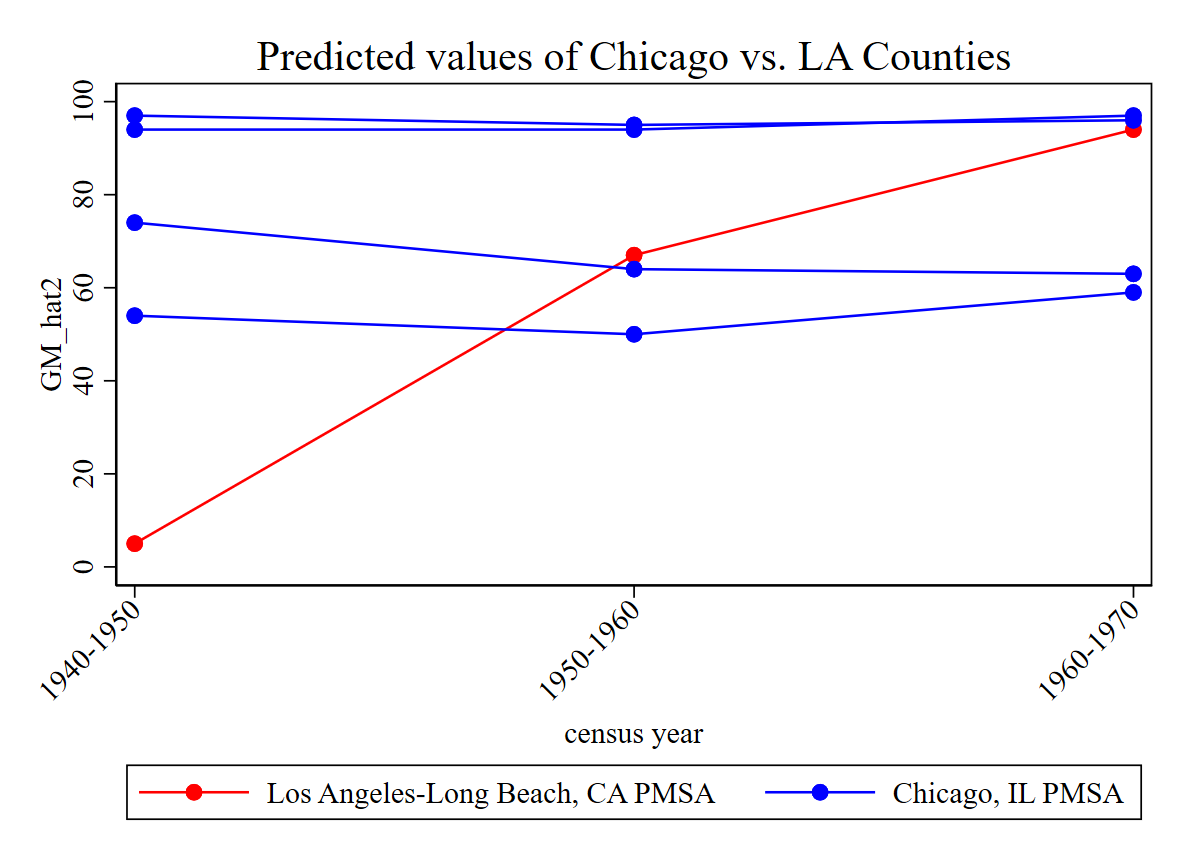
\includegraphics[width=.33\textwidth]{figures/descriptive/la_chicago_gm_hat2.png}
\end{figure}
\clearpage
\section{Goldsmith-Pinkham Table}
\begin{landscape}
{
\def\sym#1{\ifmmode^{#1}\else\(^{#1}\)\fi}
\begin{tabular}{l*{8}{c}}
\toprule
                &\multicolumn{6}{c}{County Counts Outcomes}                                               &\multicolumn{1}{c}{Directory Survey Outcomes}&\multicolumn{1}{c}{Instrument}\\\cmidrule(lr){2-7}\cmidrule(lr){8-8}\cmidrule(lr){9-9}
                &\multicolumn{1}{c}{all\_local}&\multicolumn{1}{c}{all\_local\_nosch}&\multicolumn{1}{c}{gen\_subcounty}&\multicolumn{1}{c}{gen\_muni}&\multicolumn{1}{c}{schdist\_ind}&\multicolumn{1}{c}{spdist}&\multicolumn{1}{c}{ngov3}&\multicolumn{1}{c}{GM\_hat2}\\
\midrule
base\_outcome    &      -0.23***&       0.09***&       0.01   &       0.05***&      -0.48***&       0.05   &       0.04***&              \\
                &     (0.03)   &     (0.02)   &     (0.01)   &     (0.02)   &     (0.03)   &     (0.04)   &     (0.01)   &              \\
\addlinespace
mfg\_lfshare     &       0.21** &       0.03   &       0.01*  &       0.01   &       0.02   &       0.02   &       0.01** &       0.56***\\
                &     (0.09)   &     (0.03)   &     (0.01)   &     (0.01)   &     (0.06)   &     (0.03)   &     (0.00)   &     (0.08)   \\
\addlinespace
v2\_blackmig3539\_share&      13.39** &      -0.38   &       1.36   &       0.67   &       6.03   &      -1.81   &       0.97   &      93.07***\\
                &     (6.35)   &     (3.08)   &     (1.33)   &     (1.25)   &     (4.33)   &     (3.05)   &     (0.77)   &    (15.38)   \\
\addlinespace
(sum) Pop       &       0.00** &       0.00   &       0.00*  &       0.00   &       0.00** &       0.00   &       0.00** &       0.00***\\
                &     (0.00)   &     (0.00)   &     (0.00)   &     (0.00)   &     (0.00)   &     (0.00)   &     (0.00)   &     (0.00)   \\
\addlinespace
Midwest         &      -9.09***&      -0.68   &       0.84***&       0.84***&      -0.31   &      -2.07*  &       1.50***&       5.28** \\
                &     (2.27)   &     (1.01)   &     (0.20)   &     (0.17)   &     (1.47)   &     (1.14)   &     (0.20)   &     (2.13)   \\
\addlinespace
South           &     -11.69***&      -0.40   &       0.08   &       0.22   &      -4.46   &      -3.39*  &       0.65** &     -12.93   \\
                &     (4.00)   &     (1.80)   &     (0.53)   &     (0.45)   &     (2.86)   &     (1.91)   &     (0.32)   &     (8.80)   \\
\addlinespace
West            &       6.18** &       2.71   &       1.48***&       1.51***&       4.22** &       0.10   &       2.04***&      -6.56** \\
                &     (2.83)   &     (1.75)   &     (0.46)   &     (0.33)   &     (1.79)   &     (1.41)   &     (0.31)   &     (3.23)   \\
\addlinespace
1940            &       0.00   &       0.00   &       0.00   &       0.00   &       0.00   &       0.00   &       0.00   &       0.00   \\
                &        (.)   &        (.)   &        (.)   &        (.)   &        (.)   &        (.)   &        (.)   &        (.)   \\
\addlinespace
1950            &       1.93   &       3.92***&       0.49** &       0.57** &      -7.78***&       3.60***&       0.44** &      -0.87   \\
                &     (2.52)   &     (1.15)   &     (0.24)   &     (0.23)   &     (1.61)   &     (1.19)   &     (0.17)   &     (2.14)   \\
\addlinespace
1960            &       1.89   &      -1.97** &      -0.38   &      -0.31   &      -9.18***&      -1.07   &      -0.08   &      -0.12   \\
                &     (2.10)   &     (0.89)   &     (0.24)   &     (0.22)   &     (1.53)   &     (0.86)   &     (0.13)   &     (2.33)   \\
\midrule
Observations    &     714.00   &     714.00   &     714.00   &     714.00   &     714.00   &     714.00   &     714.00   &     714.00   \\
\bottomrule
\multicolumn{9}{l}{\footnotesize Standard errors in parentheses}\\
\multicolumn{9}{l}{\footnotesize * p<0.10, ** p<0.05, *** p<0.01}\\
\end{tabular}
}

\clearpage
\end{landscape}

\section{County Comparisons: Overall}

This compares a set of "Treated" and "Control" counties in aggregate. The set is constructed by creating deciles of the county-level recent (1935-39) black migrant share of the 1940 population, then taking the counties with the largest (treated) and smallest (control) 1940-50 change in black population from each decile-census region (10 deciles x 3 regions = 30 possible pairs = 60 possible counties).The 1st and 10th deciles are dropped as the bins are constructed by frequencies, not values, thus their 1940 v2\_blackmig3539\_share values may not actually be that close. Doing this leaves us with 24 pairs/48 counties.

 These tables give summary statistics by decade on the endogenous X variable (GM), instrument (GM\_hat2), control variables (v2\_blackmig3539\_share and mfg\_lfshare), base values of outcome variables (base\_all\_local and base\_schdist\_ind), values of outcome variables (new\_all\_local and new\_schdist\_ind), and county population (countypop).

\foreach \var in {GM, GM_hat2, v2_blackmig3539_share, mfg_lfshare, base_all_local, base_schdist_ind, new_all_local, new_schdist_ind, countypop}{
	\input{tables/comparison_counties/overall_\var.tex}
}
\clearpage
\section{County Comparisons: By Region and blackmig3539\_share bins}
This section compares summary statistics for the 24 decile-census region pairs individually. 
\foreach \reg in {Northeast, Midwest, West}{
	\subsection{\reg Region}
	\foreach \bin in {1,2,3,4,5,6,7,8}{
		\input{tables/comparison_counties/byregXbin_\reg_bin_\bin.tex}
	}
	\clearpage
}

\end{document}